\documentclass{beamer}
\usepackage{amsmath}
\newcommand{\dd}{\mathop{}\!\text{d}}
\usepackage{amssymb}
\usepackage{tikz}
\usetikzlibrary{positioning}
\usefonttheme{professionalfonts}

\title{Neural Networks: From Theory to Implementation in 1 Hour}

\begin{document}

\frame{\titlepage}

\section{Why This Video?}

\begin{frame}{Why This Video?}
When I was learning machine learning, I was relying on online material and courses. The most famous one being Andrew Ng's Machine Learning Specialization and Deep Learning Specialization programs. A lot of them have two characteristics:

\begin{itemize}
    \item Start from very basics: linear regression - curve fitting with a simple line
    \item Gradually and very slowly build up towards neural networks. 
\end{itemize}

Here you learn
\begin{itemize}
    \item the theory of simple neural networks and
    \item implement them in Python.
\end{itemize}


\end{frame}

\begin{frame}{Save Time with This Video}
If you are comfortable with multiplying two matrices and applying the chain rule to get the derivative of a function, then you can deep dive into neural networks right from the beginning. This video is for you.
\end{frame}

\section{Neural Networks}

\begin{frame}{Neural Networks}
In the video, we build and train a neural network to determine whether a picture contains an image of a cat or not.

This is what a neural network looks like:

\begin{center}
\resizebox{0.5\textwidth}{!}{
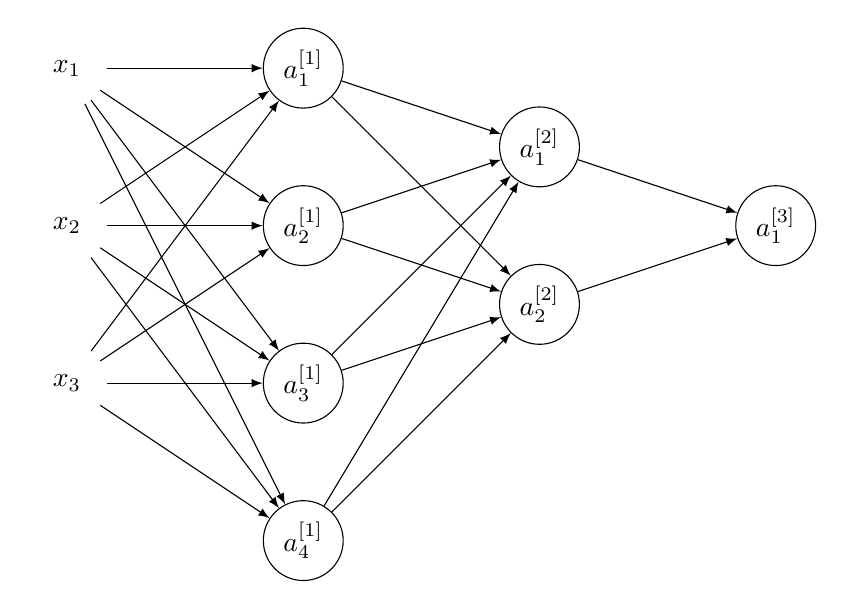
\begin{tikzpicture}[
    node distance=1.5cm and 1.5cm,
    every node/.style={circle, draw, minimum size=1cm},
    input node/.style={draw=none, minimum size=1cm},
    every path/.style={draw, -latex}
    ]

    % Nodes
    \node[input node] (x1) at (0,2) {$x_1$};
    \node[input node] (x2) at (0,0) {$x_2$};
    \node[input node] (x3) at (0,-2) {$x_3$};

    \node (h11) at (3,2) {$a^{[1]}_1$};
    \node (h12) at (3,0) {$a^{[1]}_2$};
    \node (h13) at (3,-2) {$a^{[1]}_3$};
    \node (h14) at (3,-4) {$a^{[1]}_4$};

    \node (h21) at (6,1) {$a^{[2]}_1$};
    \node (h22) at (6,-1) {$a^{[2]}_2$};

    \node (y) at (9,0) {$a^{[3]}_1$};

    % Connections
    \foreach \i in {x1, x2, x3}
        \foreach \j in {h11, h12, h13, h14}
            \path (\i) -- (\j);

    \foreach \k in {h11, h12, h13, h14}
        \foreach \l in {h21, h22}
            \path (\k) -- (\l);

    \foreach \m in {h21, h22}
        \path (\m) -- (y);

\end{tikzpicture}}
\end{center}

\end{frame}

\begin{frame}{Input Representation}
\[
X = 
\begin{pmatrix}
    x_1^{(1)} & x_1^{(2)} & \dots & x_1^{(i)} & \dots & x_1^{(m)} \\
    x_2^{(1)} & x_2^{(2)} & \dots & x_2^{(i)} & \dots & x_2^{(m)} \\
    \vdots & \vdots & & \vdots & & \vdots \\
    x_j^{(1)} & x_j^{(2)} & \dots & x_j^{(i)} & \dots & x_j^{(m)} \\
    \vdots & \vdots & & \vdots & & \vdots \\
    x_{n_x}^{(1)} & x_{n_x}^{(2)} & \dots & x_{n_x}^{(i)} & \dots & x_{n_x}^{(m)}
\end{pmatrix}
\]
\end{frame}

\section{Forward Propagation}
\begin{frame}{Forward Propagation Equations}

\[ z_j^{[l](i)} = \sum_{j'=1}^{n_{l-1}} w_{jj'}^{[l]} a_{j'}^{[l-1](i)} + b_j^{[l]} \]
\[ a_j^{[l](i)} = g^{[l]}(z_j^{[l](i)}) \quad \quad \text{Why?}\]


\[ Z^{[l]} = W^{[l]} \cdot A^{[l-1]} + b^{[l]} \]
\[ A^{[l]} = g^{[l]}(Z^{[l]}) \]
\[ (n_l,m)  = (n_l,n_{l-1}) \quad \text{Mat. Mul.} \quad (n_{l-1},m) \quad \text{Mat. Add.} \quad (n_l,m) \]
\end{frame}


\begin{frame}{Logistic Regression - Single Unit Classifier - Last Layer}
\[
J = \sum_{i=1}^{m} L^{(i)}
\]

\[
L^{(i)} = -y^{(i)} \log(a^{[L](i)}) - (1-y^{(i)}) \log(1-a^{[L](i)})
\]

\[
a^{[L](i)} = \sigma(z)
\]

\[
z_j^{[L](i)} = \sum w_{1,j'}^{[L]} a_j^{[L-1](i)} + b_j^{[L](i)}
\]

\[
\sigma(z) = \frac{1}{1+e^{-z}}
\]

\end{frame}



\begin{frame}{Gradients - Last Layer}
\[
\frac{\partial J}{\partial w_j} = \frac{\partial J}{\partial a} \cdot \frac{\partial a}{\partial z} \cdot \frac{\partial z}{\partial w_j}
\]

\[
\frac{\partial J}{\partial a} = \sum_{i=1}^{m} \left( -\frac{y  ^{(i)}   }{a} + \frac{1-y^{(i)}}{1-a} \right)
\]

\[
\frac{\partial a}{\partial z} = a(1-a)
\]

\[
\frac{\partial z}{\partial w_{1,j'}^{[L]}} = a_{j'}^{[L-1](i)}
\]

\end{frame}



\begin{frame}{Gradients - Last Layer}
\[
\frac{\partial J}{\partial w_{1,j'}^{[L]}} = \sum_{i=1}^{m} \left( a_j^{[L](i)} - y^{(i)} \right) a_j^{[L-1](i)}
\]

So for the last layer, the vectorization provides:

\[
\dd Z^{[L]} = A^{[L]}  -Y
\]

\[
\dd W^{[L]} = A^{[L-1]} \cdot {(A^{[L]}  -Y)}^T
\]


As for db, we have

\[
\frac{\partial J}{\partial b^{[L]}} = \sum_{i=1}^{m} \frac{\partial L^{(i)}}{\partial a^{[L]}}  \frac{\partial a^{[L]}}{\partial z^{[L]}}  \frac{\partial z^{[L]}}{\partial b^{[L]}}
\]

\[
\dd b^{[L]} = \sum_{\text{axis}=1} \dd Z^{L} = \sum_{\text{axis}=1} (\dd A^{L} - Y)
\]
\end{frame}




\begin{frame}{Gradients in Other Layers}
\[
\frac{\partial J}{\partial w_{jj'}^{[l]}} = \sum_{i=1}^{m} \frac{\partial L^{(i)}}{\partial a_j^{[l]}}  \frac{\partial a_j^{[l]}}{\partial z_j^{[l]}}  \frac{\partial z_j^{[l]}}{\partial w_{jj'}^{[l]}}
\]

\[
z_j^{[l](i)} = \sum_{j'=1}^{n_{l-1}} w_{jj'}^{[l]} a_{j'}^{[l-1](i)} + b_j^{[l]}
\]

\[
\frac{\partial z_j^{[l]}}{\partial w_{jj'}^{[l]}} = a_{j'}^{[l-1](i)} \quad \quad \frac{\partial a_j^{[l]}}{\partial z_j^{[l]}} = g'^{[l]}(z_j^{[l]})
\]

\[
\frac{\partial L^{(i)}}{\partial a_j^{[l]}} = \sum_{k=1}^{n_{l+1}} \frac{\partial L^{(i)}}{\partial z_k^{[l+1](i)}} \cdot \frac{\partial z_k^{[l+1](i)}}{\partial a_j^{[l](i)}}
\]

\[
\frac{\partial z_k^{[l+1](i)}}{\partial a_j^{[l](i)}} = w_{kj}^{[l+1]}
\]
\end{frame}

\begin{frame}{Gradients in Other Layers}
\[
\frac{\partial L^{(i)}}{\partial a_j^{[l]}} = \sum_{k=1}^{n_{l+1}} \frac{\partial L^{(i)}}{\partial z_k^{[l+1](i)}} w_{kj}^{[l+1]}
\]

The goal is to vectorize. So
\[
\dd A^{[l]}  =  {W^{[l+1]}}^T   \cdot   \dd Z^{[l+1]} 
\]

Remember 
\[
\frac{\partial J}{\partial w_{jj'}^{[l]}} = 
\sum_{i=1}^{m} \sum_{k=1}^{n_{l+1}} \frac{\partial L^{(i)}}{\partial z_k^{[l+1](i)}} w_{kj}^{[l+1]} \cdot 
g'^{[l]}(z_j^{[l]}) \cdot 
a_{j'}^{[l-1](i)}
\]

\[
\dd W^{[l]} (j,j') = 
\sum_{i=1}^{m}     \dd  A_j^{[l]}  g'^{[l]}(z_j^{[l]})    a_{j'}^{[l-1](i)}    
\]
\end{frame}

\begin{frame}{Gradients in Other Layers}
Assume
\[
\dd Z^{[l]}= \dd A^{[l]}  \circ  g'^{[l]}(Z^{[l]}) 
\]

So

\[
\dd  W^{[l]} (j,j') = 
\sum_{i=1}^{m}     \dd Z_{j}^{[l]}    a_{j'}^{[l-1](i)}    
\]

The goal is to vectorize. So

\[
\dd  W^{[l]}  = 
  \dd  Z^{[l]}  \cdot  {A^{[l-1]} }^T
\]
\end{frame}

\begin{frame}{Gradients in Other Layers}
\[
\frac{\partial J}{\partial w_{jj'}^{[l]}} = 
\sum_{i=1}^{m} \frac{\partial L^{(i)}}{\partial a_j^{[l]}}  
\frac{\partial a_j^{[l]}}{\partial z_j^{[l]}}  
\frac{\partial z_j^{[l]}}{\partial w_{jj'}^{[l]}}
\]

To summarize, so far we have had

\[
\dd  W^{[l]} =  (\dd  Z^{[l]} \cdot A^{[l-1]T})
\]


\[
\dd  A^{[l]} = W^{[l+1]T} \cdot \dd  Z^{[l+1]}
\]

\[
\dd  Z^{[l]} = \dd  A^{[l]} \circ g'^{[l]}(Z^{[l]})
\]
\end{frame}

\begin{frame}{Gradients in Other Layers}
\[
\frac{\partial L^{(i)}}{\partial b_j^{[l]}} = \frac{\partial L^{(i)}}{\partial z_j^{[l](i)}}  \frac{\partial z_j^{[l](i)}}{\partial b_j^{[l]}} = \dd z_j^{[l](i)}
\]

\[
\frac{\partial J}{\partial b_j^{[l]}} = \sum dZ_j^{[l]} = db^{[l]}
\]

\[
\frac{\partial L^{(i)}}{\partial b_j^{[l]}} = \frac{\partial L^{(i)}}{\partial z_j^{[l](i)}}  \frac{\partial z_j^{[l](i)}}{\partial b_j^{[l]}} = \dd Z_j^{[l](i)}; \quad \quad \frac{\partial z_j^{[l](i)}}{\partial b_j^{[l]}} = 1
\]

\[
J = \sum L^{(i)}
\]

\[
\frac{\partial J}{\partial b_j^{[l]}} = \sum \dd z_j^{[l]} = db_j^{[l]}
\]

\[
\dd  b^{[l]} = \sum_{\text{axis}=1} \dd  Z^{l}
\]
\end{frame}

\begin{frame}{Forward \& Backward Prop Summary}


\[
Z^{[l]} = W^{[l]} \cdot A^{[l-1]} + b^{[l]}
\]

\[
A^{[l]} = g^{[l]}(Z^{[l]})
\]



\[
\dd  W^{[l]} =  (\dd  Z^{[l]} \cdot A^{[l-1]T}); \quad \quad \dd W^{[L]} = A^{[L-1]} \cdot {(A^{[L]}  -Y)}^T
\]


\[
\dd  A^{[l]} = W^{[l+1]T} \cdot \dd  Z^{[l+1]}
\]

\[
\dd  Z^{[l]} = \dd  A^{[l]} \circ g'^{[l]}(Z^{[l]})
\]


\[
\dd  b^{[l]} = \sum_{\text{axis}=1} \dd  Z^{l}; \quad \quad \dd b^{[L]} = \sum_{\text{axis}=1} (\dd A^{L} - Y)
\]


%\[
%\dd  b_j^{[l]} = \sum_{i=1}^m \dd  z_j^{[l]}  
%\]

\end{frame}

\begin{frame}{Update Parameters}
\[ W^{[l]} = W^{[l]}  - \alpha \dd  W^{[l]}  \]
\[ b^{[l]} = b^{[l]}  - \alpha\dd  b^{[l]}  \]
\end{frame}








\end{document}
